%%%%%%%%%%%%%%%%%%%%%%%%%%%%%%%
\section{Introduction}
%%%%%%%%%%%%%%%%%%%%%%%%%%%%%%%

\begin{frame}{Introduction}
    What is spatio-temporal data?
    \vfill
    \begin{quote}
        Spatio-temporal data is data which contains both \textbf{time and space information}.
    \end{quote}
    \vfill
    Why spatio-temporal data?
    \vfill
    \begin{quote}
        \textbf{Large quantities} of spatio-temporal data are captured everyday by large web-based companies or industries concerned with disaster relief or marine data analysis.
        
        \medskip
        
        Spatio-temporal data is inherently \textbf{multi-dimensional} which requires creative ways to \textbf{effectively store and query} these kinds of records.
    \end{quote}
\end{frame}

\begin{frame}{Introduction}
    What is a graph database?
    \vfill
    \begin{quote}
        \textbf{Abstracts data} from a storage backend \textbf{as a graph}. Data is stored on the vertices and edges as key-value pairs.
    \end{quote}
    \vfill
    Why do we think graph databases will be more suitable?
    \vfill
    \begin{quote}
    Graph databases have been found to:
    \medskip
        \begin{itemize}
            \item Handle graph-like data more efficiently.
            \item Scale linearly with large volumes of data.
            \item Allow for concurrent, thread-local traversals.
        \end{itemize}
    \medskip
    Similar investigations have been done for \textbf{less structured} NoSQL databases and have \textbf{failed to outperform relational databases}.
    \end{quote}
\end{frame}

\begin{frame}{Introduction}
    \textbf{Final question:} How do we go about measuring suitability?
    \vfill
    \begin{itemize}
        \item Choose a suitable diversity and number of database models to compare.
        \item Apply a sufficiently large, spatio-temporal dataset.
        \item Investigate and compare each query language.
        \item Measure query response times.
        \item Investigate the guarantees of each technology with regards to ACID-compliance, CAP theorem, and real-world application.
    \end{itemize}
\end{frame}

%%%%%%%%%%%%%%%%%%%%%%%%%%%%%%%
\section{Databases}
%%%%%%%%%%%%%%%%%%%%%%%%%%%%%%%

\begin{frame}{Databases}
    Three database models were considered in this investigation:
    \vfill
    \begin{itemize}
        \item \textbf{PostgreSQL}: Open-source, relational, and object-oriented database with PostGIS extension.
        \item \textbf{JanusGraph}: Open-source graph database with Cassandra and ElasticSearch.
        \item \textbf{TigerGraph}: Enterprise-level, natively parallel, graph analytics platform.
    \end{itemize}
    \vfill
    
\includegraphics[width=.25\textwidth]{img/database-logos/postgreslogo.png}
    \hfill
    
\includegraphics[width=.25\textwidth]{img/database-logos/januslogo.png}
    \hfill
    
\includegraphics[width=.25\textwidth]{img/database-logos/tigergraph.png}database-logos/tigergraph.png
\end{frame}

%%%%%%%%%%%%%%%%%%%%%%%%%%%%%%%
\section{Dataset}
%%%%%%%%%%%%%%%%%%%%%%%%%%%%%%%

\begin{frame}{Dataset}
    The dataset applied to these databases is the \textbf{Yelp Challenge Dataset}\parnote{\url{www.yelp.com/dataset/challenge/}}.
    \vfill
    \begin{columns}
        \begin{column}{.6\textwidth}
        The dataset contains
            \begin{itemize}
                \item \textbf{coordinates} of each business,
                \item the \textbf{timestamps} of each review, and
                \item users and their friend relations.
            \end{itemize}
            \end{column}%
            \hfill%
            \begin{column}{.39\textwidth}
            \centering
            
\includegraphics[width=0.7\columnwidth]{img/yelp-logo.png}
        \end{column}%
    \end{columns}
    \vfill
    This makes for a strongly connected, dense, \textbf{graph-like} dataset with an additional social aspect. The queries are expected to be \textbf{complex, multi-join style} queries.
    \vfill
    \parnotes
\end{frame}

%%%%%%%%%%%%%%%%%%%%%%%%%%%%%%%
\section{Challenges}
%%%%%%%%%%%%%%%%%%%%%%%%%%%%%%%

\begin{frame}{Challenges}
    The following are some the challenges faced in this investigation:
    \vfill
    \begin{columns}
        \begin{column}{.6\textwidth}
            \begin{itemize}
                \item Learning the NoSQL database domain and each technology.
                \item Writing complex queries in each query language.
                \item Database design.
                \item Applying suitable, real-world data analysis.
                \item Multi-dimensional indexing.
                \item Hardware limitations.
            \end{itemize}
            \end{column}%
            \hfill%
            \begin{column}{.39\textwidth}
            \centering
            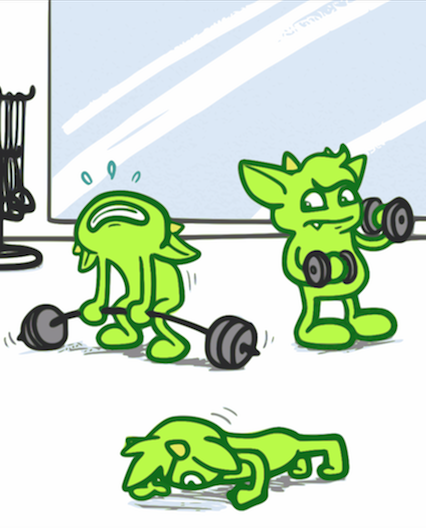
\includegraphics[width=0.7\columnwidth]{img/gremlin-images/gremlin-gym-crop.png}
        \end{column}%
    \end{columns}
    \vfill
    A number of technologies and programming languages had to be learned in order to perform the investigation.
    \vfill
    \parnotes
\end{frame}

%%%%%%%%%%%%%%%%%%%%%%%%%%%%%%%
\section{NoSQL}
%%%%%%%%%%%%%%%%%%%%%%%%%%%%%%%

\begin{frame}{NoSQL}
    In order of least to most structured:
    \vfill
    \begin{tabular}{p{2.4cm}|p{7.5cm}}
        \textbf{Category} & \textbf{Description} \\
        \hline
        \hline
        Key-value store & Keys as identifiers to values as a data object or collection of data objects. \\
        \hline
        Document store & A key-value store but values are document types e.g. JSON, XML. Both keys and values are fully searchable. \\
        \hline
        Column family & Store data along columns as column-families. Column-families are grouped together in keyspaces. \\
        \hline
        Graph & Graph abstraction of storage backend. Backed usually a column-family store or relational database.\\
    \end{tabular}
    \vfill
    NoSQL aims to relax on consistency constraints to improve \textbf{partition tolerance} and \textbf{availability}.
\end{frame}

%%%%%%%%%%%%%%%%%%%%%%%%%%%%%%%
\section{Graph Query Languages}
%%%%%%%%%%%%%%%%%%%%%%%%%%%%%%%

\begin{frame}{Graph Query Languages}
    The following graph query languages were considered:
    \vfill
    \begin{itemize}
        \item \textbf{Gremlin}: The traversal language of Apache TinkerPop.
        \item \textbf{Cypher}: Graph pattern matching language by Neo4j.
        \item \textbf{GSQL}: TigerGraph's graph query language.
    \end{itemize}
    \vfill
    
\includegraphics[width=.25\textwidth]{img/graph-lang/gremlin-running.png}
    \hfill
    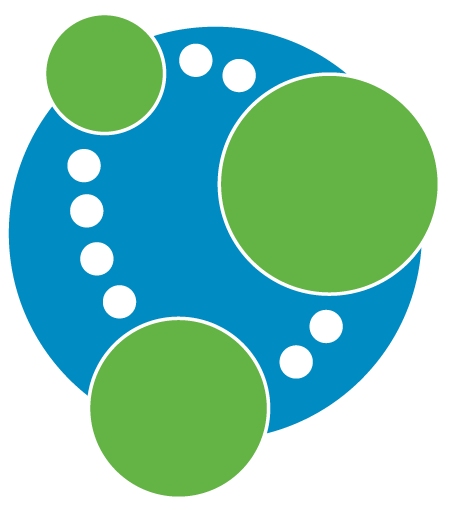
\includegraphics[width=.25\textwidth]{img/graph-lang/neo4j.png}
    \hfill
    
\includegraphics[width=.25\textwidth]{img/database-logos/tigergraph.png}
\end{frame}

\begin{frame}{Gremlin}
    \begin{columns}
        \begin{column}{.6\textwidth}
            \begin{itemize}
                \item Functional, data-flow query language.
                \item Integrates with multiple vendors e.g. JanusGraph.
                \item Queries can be both imperative or declarative.
                \item Embeds itself into host programming language.
                \item Turing-complete.
            \end{itemize}
            \end{column}%
            \hfill%
            \begin{column}{.39\textwidth}
            \centering
            
\includegraphics[width=0.7\columnwidth]{img/graph-lang/gremlin-running.png}
        \end{column}%
    \end{columns}
\end{frame}

\begin{frame}{Gremlin}
    An example of imperative Gremlin in this project:
    \lstinputlisting[
    language=gremlin,
    caption={
        A Gremlin query that returns all the IDs of all the users who have rated restaurants a user has been to above 3 stars.
    },
    label={lst:gremlin1}
    ]
    {./queries/kate.groovy}
\end{frame}

\begin{frame}{Cypher}
    \begin{columns}
        \begin{column}{.6\textwidth}
            \begin{itemize}
                \item Declarative pattern matching query language.
                \item Can compile into other graph query languages e.g. Gremlin, GSQL.
                \item Makes use of ASCII-art in syntax.
                \item SQL-like and aims to be concise and easy to learn.
                \item Not Turing-complete.
            \end{itemize}
            \end{column}%
            \hfill%
            \begin{column}{.39\textwidth}
            \centering
            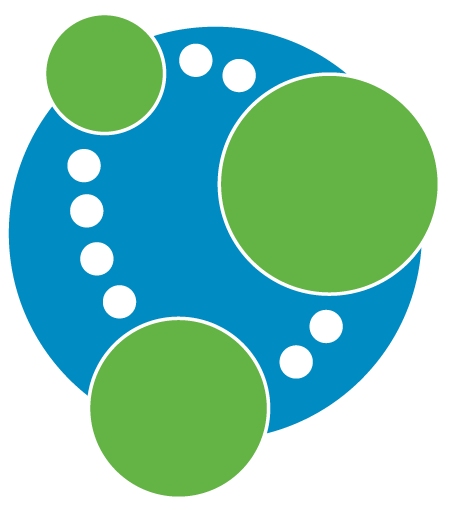
\includegraphics[width=0.7\columnwidth]{img/graph-lang/neo4j.png}
        \end{column}%
    \end{columns}
\end{frame}

\begin{frame}{Cypher}
    An example of an application of Cypher on this dataset:
\lstinputlisting[
    language=cypher,
    caption={Returns all users who have reviewed the same businesses as a given user. The query iterates through all users. Note how the return match verifies that the user \texttt{p1} does not match user \texttt{p2}.}
    ]
    {./queries/reviews.cql}
\end{frame}

\begin{frame}{GSQL}
    \begin{columns}
        \begin{column}{.6\textwidth}
            \begin{itemize}
                \item SQL-like language that takes after Gremlin and Cypher.
                \item Queries can be both imperative or declarative.
                \item Can accumulate data simultaneously.
                \item Procedural and parameterized queries.
                \item Turing-complete.
            \end{itemize}
            \end{column}%
            \hfill%
            \begin{column}{.39\textwidth}
            \centering
            
\includegraphics[width=0.7\columnwidth]{img/database-logos/tigergraph.png}
        \end{column}%
    \end{columns}
\end{frame}

\begin{frame}{GSQL}
    An example of the GSQL implementation of Listing \ref{lst:gremlin1}.
\lstinputlisting[
    language=gsql,
    caption={A Gremlin query that returns all the IDs of all the users who have rated restaurants a user has been to above 3 stars.},
    label={lst:gsql1}
    ]
    {./queries/kate1-1.gsql}
\end{frame}

\begin{frame}{GSQL}
    Listing \ref{lst:gsql1} continued.
\lstinputlisting[
    language=gsql,
    caption={A Gremlin query that returns all the IDs of all the users who have rated restaurants a user has been to above 3 stars.}
    ]
    {./queries/kate1-2.gsql}
\end{frame}